\documentclass{article}
\usepackage{tikz}
\usepackage[pass,paperwidth=4cm,paperheight=4cm]{geometry}
\definecolor{darkgreen}{RGB}{0,192,0}
\title{Cartesian closed categories and the price of eggs}
\author{Jane Doe}
\date{September 1994}
\begin{document}

	\usetikzlibrary{arrows.meta}
	\tikzset{>={Latex[width=3mm,length=3mm]}}

	% bezier curve diagram
	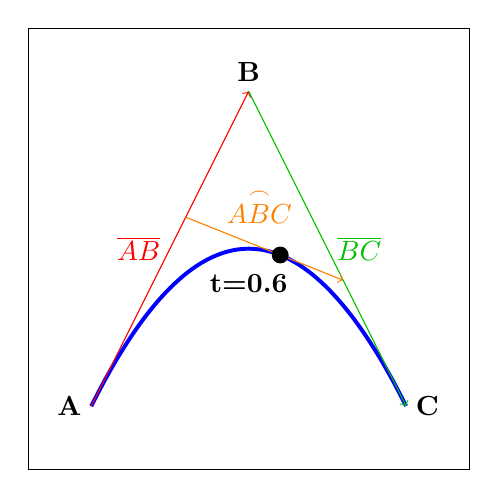
\begin{tikzpicture}[x=4cm,y=4cm]
		% border
		\draw (-0.2,-0.2) -- (1.2,-0.2) -- (1.2,1.2) -- (-0.2,1.2) -- (-0.2,-0.2);
		% 1d quadratic bezier curve with control points 0,1,0
		\draw[scale=1,domain=0:1,smooth,variable=\x,blue,line width=0.5mm] plot ({\x},{2*\x-2*\x*\x});		
		% control polygon / labels
		\draw[red,->]       (0.0,0.0) -- (0.5,1.0);
		\draw[darkgreen,->] (0.5,1.0) -- (1.0,0.0);
		\draw[red]          (0.25,0.5) node[anchor=east] {$\overline{AB}$};
		\draw[darkgreen]    (0.75,0.5) node[anchor=west] {$\overline{BC}$};
		% control point labels
		\draw (0.0,0.0) node[anchor=east]  {\bf{A}};
		\draw (0.5,1.0) node[anchor=south] {\bf{B}};
		\draw (1.0,0.0) node[anchor=west]  {\bf{C}};
		% draw a line from AB->AC for time = 0.75
		\draw[orange,->] (0.3,0.6) -- (0.8,0.4);
		\draw[orange] (0.40,0.55) node[anchor=south west] {$\stackrel{\frown}{ABC}$};
		% draw the point at t=0.6 and label underneath the curve
		\draw[black,fill=black] (0.6,0.48) circle (1mm);
		\draw[black] (0.5,0.45) node[anchor=north] {\bf{t}=0.6};
	\end{tikzpicture}
	% bilinear diagram
	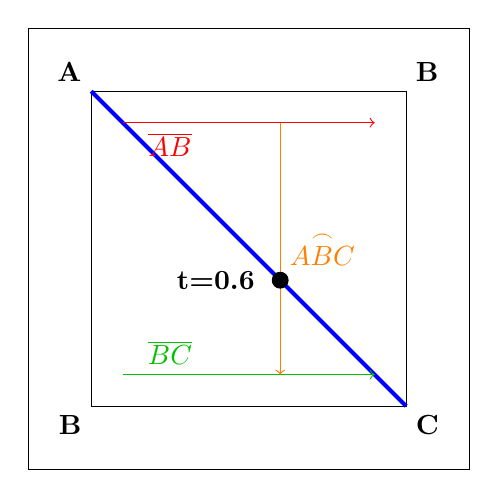
\begin{tikzpicture}[x=4cm,y=4cm]
    	% border
    	\draw (-0.2,-0.2) -- (1.2,-0.2) -- (1.2,1.2) -- (-0.2,1.2) -- (-0.2,-0.2);
    	% box
    	\draw (0,0) -- (1,0) -- (1,1) -- (0,1) -- (0,0);
    	% representative line for where the quadratic bezier curve lives
    	\draw[blue,line width=0.5mm] (0,1) -- (1,0);		
    	% corner labels
    	\draw (0,1) node[anchor=south east] {\bf{A}};
    	\draw (1,1) node[anchor=south west] {\bf{B}};    	
    	\draw (0,0) node[anchor=north east] {\bf{B}};
    	\draw (1,0) node[anchor=north west] {\bf{C}};
    	% x axis interpolation
    	\draw[red,->]       (0.1,0.9) -- (0.9,0.9);
    	\draw[red]          (0.25,0.9) node[anchor=north] {$\overline{AB}$};
    	\draw[darkgreen,->] (0.1,0.1) -- (0.9,0.1);
    	\draw[darkgreen]    (0.25,0.1) node[anchor=south] {$\overline{BC}$};
    	% y axis interpolation
    	\draw[orange,->]    (0.6,0.9) -- (0.6,0.1);
    	\draw[orange]    	(0.6,0.5) node[anchor=west] {$\stackrel{\frown}{ABC}$};
    	% draw the point at t=0.6 and label for it
    	\draw[black,fill=black] (0.6,0.4) circle (1mm);
    	\draw[black] (0.55,0.4) node[anchor=east] {\bf{t}=0.6};
    	
	\end{tikzpicture}	

\end{document}